\documentclass[a4paper, 12pt]{article}%тип документа

%%%Библиотеки
	%\usepackage[warn]{mathtext}	
	\usepackage[T2A]{fontenc} % кодировка
	\usepackage[utf8]{inputenc} % кодировка исходного текста
	\usepackage[english,russian]{babel} % локализация и переносы
	\usepackage{caption}
	\usepackage{listings}
	\usepackage{amsmath,amsfonts,amssymb,amsthm,mathtools}
	\usepackage{wasysym}
	\usepackage{graphicx}%Вставка картинок правильная
	\usepackage{float}%"Плавающие" картинки
	\usepackage{wrapfig}%Обтекание фигур (таблиц, картинок и прочего)
	\usepackage{fancyhdr} %загрузим пакет
	\usepackage{lscape}
	\usepackage{xcolor}
	\usepackage[normalem]{ulem}
	\usepackage{hyperref}

%%%Конец библиотек




%%%Настройка ссылок
	\hypersetup
	{
		colorlinks=true,
		linkcolor=blue,
		filecolor=magenta,
		urlcolor=blue
	}
%%%Конец настройки ссылок


%%%Настройка колонтитулы
	\pagestyle{fancy}
	\fancyhead{}
	\fancyhead[L]{Лабораторная работа}
	\fancyhead[R]{Талашкевич Даниил, группа Б01-008}
	\fancyfoot[C]{\thepage}
%%%конец настройки колонтитулы



							\begin{document}
						%%%%Начало документа%%%%


%%%Начало титульника
\begin{titlepage}

	\newpage
	\begin{center}
		\normalsize Московский физико-технический институт \\(госудраственный 			университет)
	\end{center}

	\vspace{6em}

	\begin{center}
		\Large Лабораторная работа по квантовой физике\\
	\end{center}

	\vspace{1em}

	\begin{center}
		\large \textbf{Исследование эффекта Комптона [1.2]}
	\end{center}

	\vspace{2em}

	\begin{center}
		\large Талашкевич Даниил Александрович\\
		Группа Б01-008
	\end{center}

	\vspace{\fill}

	\begin{center}
	Долгопрудный \\2022
	\end{center}
	
\end{titlepage}
%%%Конец Титульника



%%%Настройка оглавления и нумерации страниц
	\thispagestyle{empty}
	\newpage
	\tableofcontents
	\newpage
	\setcounter{page}{1}
%%%Настройка оглавления и нумерации страниц


					%%%%%%Начало работы с текстом%%%%%%

\section{Аннотация}

\ \ \ \ \textbf{Цель работы:} исследование энергетического спектра $\gamma$-квантов, рассеянных на графите, с помощью сцинтилляционного спектрометра, определение энергии рассеянных $\gamma$-квантов в зависимости от угла рассеяния, определение энергии покоя частиц, на которых происходит комптоновское рассеяние.

\textbf{В работе используются:} источник излучения, графитовая мишень, сцинтилляционный счётчик, ФЭУ, ЭВМ

\section{Теоретические положения}
\textbf{Эффект Комптона} - увеличение длины волны рассеянного излучения по сравнению с падающим. Он интерпретируется как результат упругого соударения двух частиц - $\gamma$-кванта и свободного электрона. \par
Пусть электрон до соударения покоился, а  $\gamma$-квант имел начальную энергию $\omega_0$ и импульс $\omega_0/c$. После соударения электрон приобретает энергию $\gamma mc^2$, где $\gamma = (1 - \beta^2)^{-1/2}$, $\beta = v/c$, а  $\gamma$-квант рассеивается на некоторый угол $\theta$ по отношению
к первоначальному направлению движения. Энергия и импульс рассеянного излучения — $\propto \omega_1$. Запишем для рассматриваемого процесса законы сохранения энергии и импульса:

\begin{equation}
    mc^2 +\hbar \omega_0 = \gamma mc^2 +\hbar \omega_1
\label{1eq}
\end{equation}

\begin{center}
    $\frac{\hbar \omega_0}{c} = \gamma mv \cos \varphi + \frac{\hbar \omega_1}{c} \cos \theta$ \\
    $\gamma mv \sin \varphi = \frac{\hbar \omega_1}{c} \sin \theta$
\end{center}
Решая совместно эти уравнения и переходя от частот к длинам волн, получаем изменение длины рассеянного излучения
\begin{equation}
    \triangle \lambda = \lambda_1 - \lambda_0 = \frac{h}{mc}(1 - \cos \theta) = \Lambda_k(1 - \cos \theta),
\label{eq1}
\end{equation}
где $\Lambda_k = \frac{h}{mc} = 2.42 \dot 10^{-10}$ см - комптоновская длина волны электрона. \par
Основной целью работы является проверка соотношения (1). Преобразуем его от длин волн к энергии $\gamma$-квантов:
\begin{equation}
    \frac{1}{\varepsilon(\theta)} - \frac{1}{\varepsilon_0} = 1 - \cos \theta,
    \label{eq2}
\end{equation}
где $\varepsilon_0 = E_0/(mc^2)$ - энергия $\gamma$-квантов, падающих на рассеиватель (в единицах $mc^2$), $\varepsilon(\theta)$ - выраженная в тех же единицах энергия квантов, испытавших комптоновское рассеяния на угол $\theta$, $m$ - масса электрона.

\section{Экспериментальная установка}

        \begin{figure}[h]
\begin{center}
\begin{minipage}[h]{0.48\linewidth}
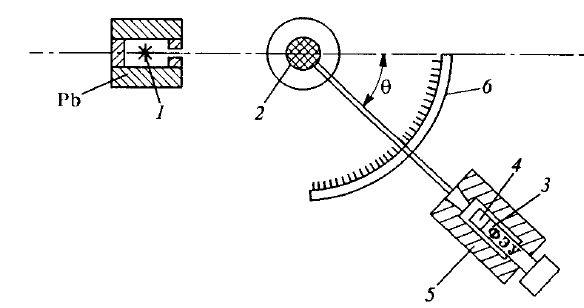
\includegraphics[width=1\linewidth]{fig2.PNG}
\caption{Блок-схема установки по изучению рассеяния $\gamma$-квантов} %% подпись к рисунку\label{ris:experimoriginal} %% метка рисунка для ссылки на него
\end{minipage}
\hfill 
\begin{minipage}[h]{0.48\linewidth}
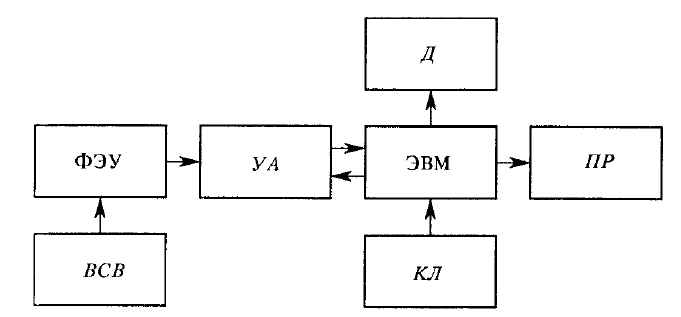
\includegraphics[width=1\linewidth]{fig3.PNG}
\caption{Блок-схема измерительного комплекса}
\label{ris:experimcoded}
\end{minipage}
\end{center}
\end{figure}

Источником излучения служит $^{137}$Cs(1), испускающий  $\gamma$-кванты с энергией 662 кэВ. Узкий пучок после коллиматора попадает на графитовую мишень (2). Кванты, испытавшие комптоновское рассеяния в мишени, регистрируются сцинтилляционным счетчиком и проходят на ФЭУ. Сигналы, возникающие на ФЭУ, подаются на ЭВМ для амплитудного анализа. Штанга с измерительным блоком может вращаться относительно мишени.


\section{Ход работы}

\begin{figure}[!h]
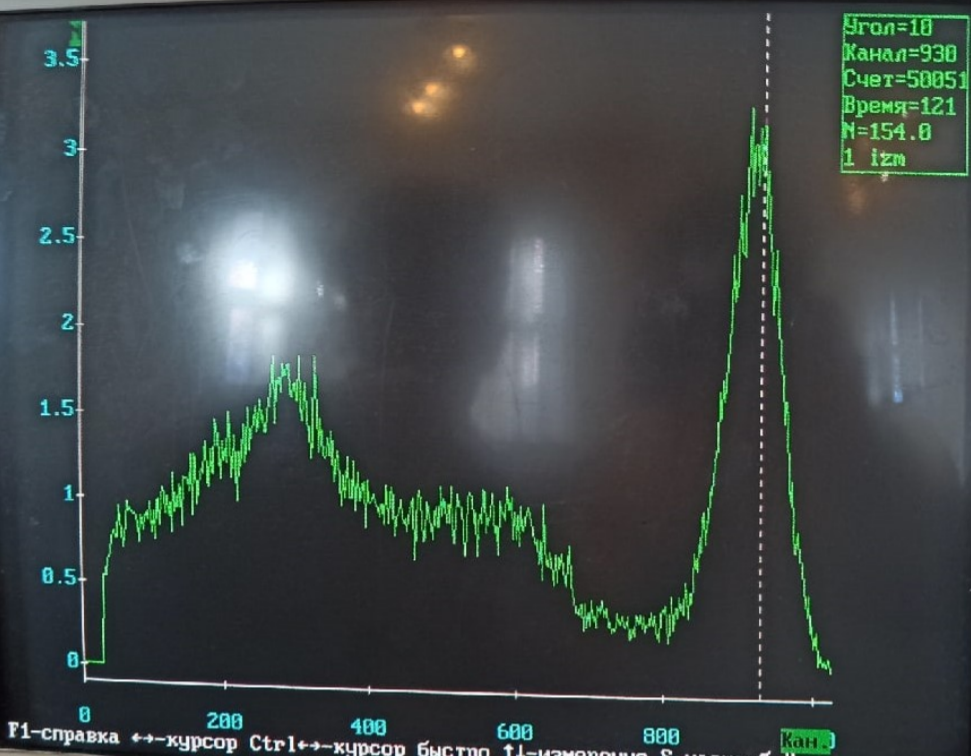
\includegraphics[width = 0.9\textwidth]{4.png}
\centering
\caption{Наблюдаемая на дисплее компьютера картина.}
\end{figure}

Устанавливая сцинтилляционный счётчик под разными углами $\theta$, произведём измерения, каждое примерно по десять минут, отмечая, какому каналу соответствует фотопик при каждом значении угла. Картина, наблюдаемая на дисплее компьютера, представлена на Рис. 3
Результаты измерений представлены в Таблице 1, как отмечалось выше, погрешнсть измерения канала -- 1\%, так как она для всех измерений больше, чем половина расстояния до соседнего возможного пика, учитывалась только она, погрешность измерения угла $\theta$ берём ценой деления лимба $\sigma_\theta = 2^\circ$.
\begin{table}[h]
\begin{tabular}{|c|c|c|c|c|c|c|c|c|c|c|c|c|c|}
\hline
$\theta$, $^\circ$ & 0   & 10  & 20  & 30  & 40  & 50  & 60  & 70  & 80  & 90  & 100 & 110 & 120 \\ \hline
$N$                & 931 & 918 & 819 & 784 & 713 & 608 & 533 & 471 & 417 & 382 & 352 & 319 & 311 \\ \hline
$\sigma_N$         & 9   & 9   & 8   & 8   & 7   & 6   & 5   & 5   & 4   & 4   & 4   & 3   & 3   \\ \hline
\end{tabular}
\centering
\caption{Результаты измерений.}
\end{table}
По этим данным постоим график зависимости $1/N(\theta)$ от $1-\cos \theta$ (Рис. 4). Здесь погрешности считали по формулам
\[\begin{array}{l}
\sigma_{1/N} = \dfrac{\sigma_N}{N^2},\\
\sigma_{1-\cos \theta} = \sin(\theta) \sigma_\theta.\\
\end{array}\]
Заметим, что во все формулы $\theta$ и $\sigma_\theta$ подставляется в радианах. Из графика по МНК получим угловой коэффициент, в соответствии с \eqref{1b} равный $A$, и точку пересечения с осью ординат, соответветствующую $1/N(0)$. Формулы расчёта (здесь $x = 1 -\cos\theta$ и $y = 1/N$):
\[\begin{array}{l l}
A = \dfrac{\langle xy \rangle - \langle x \rangle \langle y \rangle}{\langle x^2 \rangle - \langle x \rangle^2}, & \sigma_A = \dfrac{1}{\sqrt{n}}\sqrt{\dfrac{\langle y^2 \rangle - \langle y \rangle^2}{\langle x^2 \rangle - \langle x \rangle^2} - A^2},\\
\dfrac{1}{N(0)} = \langle y \rangle - A \langle x \rangle, & \sigma_{1/N(0)} = \sigma_A \sqrt{\langle x^2\rangle},\\
\end{array}\]
где $\langle \cdot \rangle$ обозначает среднее значение, $n = 13$ -- число опытов.
\begin{figure}[h]
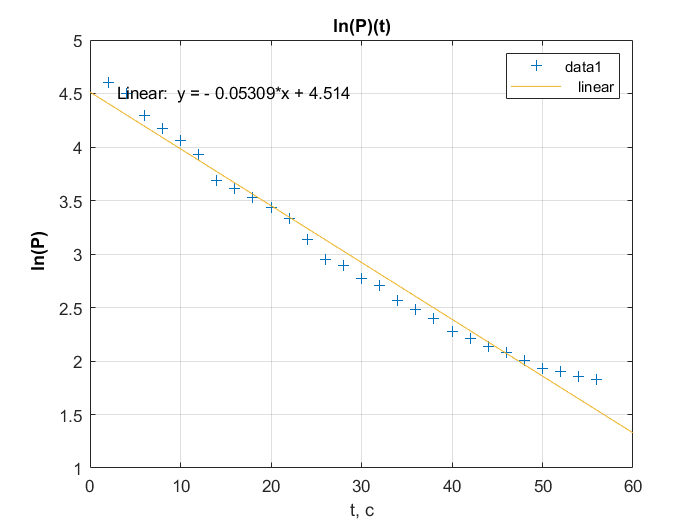
\includegraphics[width = 0.7\textwidth]{fig1.png}
\centering
\caption{График зависимости $1/N$ от $1-\cos \theta$.}
\end{figure}


Из аппроксимации получим <<наилучшие>> значения каналов для $\theta = 0^\circ$ и $\theta = 90^\circ$:
\[\begin{array}{l}
N_{\text{наил}}(0) = \dfrac{1}{\frac{1}{N(0)}} = 920 \pm 20,\\[12pt]
N_{\text{наил}}(90) = \dfrac{1}{\frac{1}{N(0)}+A} = 384 \pm 7,\\
\end{array}
\]
где погрешности считались по формулам
\[
\begin{array}{l}
\sigma_{N_{\text{наил}}(0)} = \dfrac{\sigma_{\frac{1}{N(0)}}}{(\frac{1}{N(0)})^2},\\[14pt]
\sigma_{N_{\text{наил}}(90)} = \dfrac{\sigma_{\frac{1}{N(0)}} + \sigma_{A}}{(\frac{1}{N(0)}+A)^2}.\\
\end{array}
\]
Наконец, по формуле \ref{1eq} (для $N(0)$ и $N(90)$ брались наилучшие значения) получим энергию покоя электрона
\[mc^2 = 480 \pm 20~\text{кэВ},\]
погрешность считалась по формуле
\[\sigma_{mc^2} = \sqrt{ \left( \dfrac{\partial (mc^2)}{\partial N_{\text{наил}}(0)} \right)^2 \sigma_{N_{\text{наил}}(0)}^2 +\left( \dfrac{\partial (mc^2)}{\partial N_{\text{наил}}(90)} \right)^2 \sigma_{N_{\text{наил}}(90)}^2 }\]
Здесь использовалось, что $E_\gamma = 662~\text{кэВ}$ (значение взято из \cite{laba}). Истинная энергия покоя электрона 510 кэВ лежит в двух сигмах от полученного результата.

\section{Вывод}

Итак, в настоящей лабораторной работе нами была проведена проверка соотношения (\ref{eq1}). Экспериментально установлено, что $\gamma$-кванты действительно испытывают упругое рассеяние на свободных частицах. 
	
	Обратим наше внимание на то, что с увеличением угла $\theta$ погрешность измерения номера канала $\sigma_N$ увеличивается, что связано со смещением фотопика в сторону сплошного распределения, обязанного комптоновскому рассеянию. При $\theta = 110^\circ$ уже было невозможно увидеть пик полного поглощения.
	
	На основании полученных данных можно определить энергию покоя частиц, на которых происходит комптоновское рассеивание. Путем несложных преобразований формула (\ref{eq2}) принимает вид:
	\begin{equation*}
		mc^2 = E(0) \frac{N_\text{наил}(90)}{N_\text{наил}(0)-N_\text{наил}(90)},
	\end{equation*}
	где $E(0)$ -- энергия $\gamma$-лучей, испускаемых источником (в нашем случае $^{137}$Cs), то есть 662 кэВ. Имеем:
	\[
	\boxed{mc^2 = 430 \pm 20 \ \text{кэВ}}.
	\]
	Видно, что результат на 16\% меньше 511 кэВ -- энергии покоя электрона. Почему? Погрешность должна быть больше...
	
	Отметим, что колебания напряжения на ФЭУ № 4012 практически не вносят погрешности в измерения, ведь в работе было использовано напряжение $U = 1,6$ кэВ, при котором счетная характеристика выходит на константу, как видно из рисунка~\ref{fig:U}.
	
\begin{thebibliography}{9}
\bibitem{laba} 
Игошин Ф.Ф., Самарский Ю.А., Ципенюк Ю.М. 
\textit{Лабораторный практикум по общей физике: Учеб. пособие для вузов. Т. 3 Квантовая физика}. 
М.: Физматкнига, 2005.
\end{thebibliography}


\end{document}
